% arara: pdflatex: { shell: yes }
% arara: pythontex: {verbose: yes, rerun: modified }
% arara: pdflatex: { shell: yes }
% arara: move: {  files: ['assignments.pdf'], target: ['../pdf-files'] }


\documentclass[a4paper,12pt]{article}


%\usepackage[nosolutions]{optional}
%\usepackage[justhints]{optional}
%\usepackage[check]{optional}
\usepackage[all-solutions-at-end]{optional}

\usepackage{../common/preamble}
%\newcommand{\sectionbreak}{\clearpage}
\setcounter{tocdepth}{2}
\usepackage{a4wide}
\usepackage{../common/abbreviations}


\newtheorem{theorem}{Theorem}[section]
\newtheorem{exercise}[theorem]{Ex}
\newtheorem{remark}[theorem]{Remark}


% \Opensolutionfile{hint}
% \Opensolutionfile{ans}



\author{PD team}
\date{\today}
\title{Probability distributions EBP038A05\\
Assignments}

\begin{document}
\maketitle
\tableofcontents

\subfile{PT_main-assignments.tex}

\subfile{intro.tex}


\section{Assignment 1}
\subfile{bh-5-exp.tex}
\subfile{bh-5-6-5.tex}
\subfile{bh-7-1.tex}
\subfile{bh-7-9.tex}


\section{Assignment 2}
\subfile{bh-7-48.tex}
\subfile{bh-7-53.tex}
\subfile{bh-7-86.tex}


\section{Assignment 3}
\subfile{bh-8-4-figure.tex}
\subfile{bh-8-4-3.tex}
\subfile{bh-8-1.tex}
\subfile{bh-8-18.tex}



\section{Assignment 4}
\subfile{bh-8-27.tex}
\subfile{bh-8-36.tex}
\subfile{bh-8-54.tex}
\subfile{bh-9-1.tex}


\section{Assignment 5}
\subfile{bh-9-1-7.tex}
\subfile{bh-9-1-9.tex}
\subfile{bh-9-6-1.tex}
\subfile{bh-9-7.tex}



\section{Assignment 6}
\subfile{bh-9-25.tex}
\subfile{bh-9-37.tex}
\subfile{bh-9-50.tex}
\subfile{bh-10-2-3.tex}


\section{Assignment 7}
\subfile{bh-10-9.tex}
\subfile{bh-10-28.tex}
\subfile{bh-10-30.tex}
\subfile{bh-10-39.tex}

\clearpage
\section{Challenges}
These problems are for fun, but not needed for the exam. You won't get extra points for it. However, from past years we know that the good students really liked these challenges.
\subfile{poisson.tex}
\subfile{cauchy.tex}
\subfile{records.tex}
\subfile{normal.tex}
\subfile{recourse.tex}
\subfile{beluga.tex}
\subfile{benford.tex}
\subfile{betting.tex}




% \opt{justhints}{
% \Closesolutionfile{hint}
% \clearpage
% \section{Hints}
% \begin{Hint}{1.2}
			Note the difference between mean and median. This question sheds light on the link between our informal daily languages and formal mathematical concepts.
		
\end{Hint}
\begin{Hint}{1.5}
			For the median, use the fact that the Cauchy density function is symmetric about $0$.
		
\end{Hint}
\begin{Hint}{1.6}
			Given any random variable $X$ whose distribution is symmetric about some point $\mu$, you can construct a random variable $Y$ that is symmetric about 0. What can you say about $E(Y^3)$ and $E((-Y)^3)$?
		
\end{Hint}
\begin{Hint}{1.7}
			Check from the definition that a random variable $X$ has zero skewness if $E(X) = E(X^3) = 0$. Construct a random variable satisfying this property. The easiest option is to consider a discrete random variable with 3 values in its support.
		
\end{Hint}
\begin{Hint}{1.9}
			Note that variances (if exist) are always non-negative.
%			\textbf{Intuition:} ${\displaystyle \operatorname {E} (X)=\operatorname {P} (X<a)\cdot \operatorname {E} (X|X<a)+\operatorname {P} (X\geq a)\cdot \operatorname {E} (X|X\geq a)}$ where ${\displaystyle \operatorname {E} (X|X<a)}$  is larger than 0 as r.v. ${\displaystyle X}$ is non-negative and ${\displaystyle \operatorname {E} (X|X\geq a)}$  is larger than ${\displaystyle a}$ because the conditional expectation only takes into account of values larger than ${\displaystyle a}$ which r.v. ${\displaystyle X}$ can take. Hence intuitively ${\displaystyle \operatorname {E} (X)\geq \operatorname {P} (X\geq a)\cdot \operatorname {E} (X|X\geq a)\geq a\cdot \operatorname {P} (X\geq a)}$${\displaystyle \operatorname {E} (X)\geq \operatorname {P} (X\geq a)\cdot \operatorname {E} (X|X\geq a)\geq a\cdot \operatorname {P} (X\geq a)}$, which directly leads to ${\displaystyle \operatorname {P} (X\geq a)\leq {\frac {\operatorname {E} (X)}{a}}}$.
		
\end{Hint}
\begin{Hint}{1.10}
		\begin{enumerate}[i.]
			\item Use the fundamental bridge. Note that
			\begin{equation*}
				\begin{array}{cl}
						P(|X-\mu|\geq \epsilon) &= E(1_{\{\left( |X-\mu|\geq \epsilon\right) \}})= E(1_{\{  \frac{|X-\mu|}{\epsilon}\geq 1  \}})
				\end{array}
			\end{equation*}
		\item Show that $1_{\{ \frac{|X-\mu|}{\epsilon}\geq 1  \}}\leq \left( \frac{|X-\mu|}{\epsilon}\right)^2 $.
		\item The above two imply that $P(|X-\mu|\geq \epsilon)\leq E\left( \frac{|X-\mu|}{\epsilon}\right)^2$.
		\end{enumerate}
	
\end{Hint}
\begin{Hint}{1.12}
			Use the result from Ex \ref{ex:chap06:05}.
		
\end{Hint}
\begin{Hint}{1.13}
			First, derive the identity $\sum_{i = 1}^n (X_i - \mu)^2 = \sum_{i = 1}^n (X_i - \bar{X}_n)^2 + n (\bar{X}_n - \mu)^2$.
		
\end{Hint}
\begin{Hint}{1.14}
		Try to make use the fact that sample average of i.i.d. data goes to the expectation by decomposing $S^2$ as the sum of components with sample averages.  $$S_n^2 = \frac{n}{n - 1}\frac{1}{n} \sum_{i = 1}^n (X_i - \mu)^2 - \frac{n}{n - 1} (\bar{X}_n - \mu)^2.$$
	
\end{Hint}
\begin{Hint}{1.15}
			If you were to throw a fair coin a large number of times, what is the proportion of heads you would expect?
		
\end{Hint}
\begin{Hint}{1.16}
			FUse that if $X \sim N(\mu, \sigma^2)$, the MGF of $X$ is given by $M_X(t) = e^{\mu t} e^{\frac{1}{2} \sigma^2 t^2}$.
		
\end{Hint}
\begin{Hint}{1.18}
			Recall the formula for geometric series: for $|\rho| < 1$, $\sum_{k = 0}^{\infty} \rho^k = \frac{1}{1 - \rho}$.
		
\end{Hint}
\begin{Hint}{1.19}
			For $X \sim N(\mu, \sigma^2)$, the MGF of $X$ is given by $M_X(t) = e^{\mu t} e^{\frac{1}{2} \sigma^2 t^2}$. Now take derivatives.
		
\end{Hint}
\begin{Hint}{1.20}
			For $X \sim N(\mu, \sigma^2)$, the MGF of $X$ is given by $M_X(t) = e^{\mu t} e^{\frac{1}{2} \sigma^2 t^2}$. Now take derivatives.
		
\end{Hint}
\begin{Hint}{1.21}
		MGFs determines distributions. Show the MGF of the sum can not be written in the form of the Expo MGF.
	
\end{Hint}
\begin{Hint}{1.22}
		MGF!
	
\end{Hint}
\begin{Hint}{1.23}
		MGF!
	
\end{Hint}
\begin{Hint}{1.24}
		The sum of independent Gaussian is Gaussian, use the fact that $X_1+X_2\sim N(\mu_1+\mu_2, \sigma_1^2+\sigma_2^2)$ when $X_1,X_2$ are independent and $X_i\sim N(\mu_i, \sigma_i^2), i=1,2$.
	
\end{Hint}
\begin{Hint}{1.28}
		MGF!
	
\end{Hint}

% \begin{Solution}{1.1}
			Let $X = 10^{100} B$, where $B \sim \text{Bern}(10^{-10})$. The mean $\mu$ of $X$ is $10^{100} \cdot 10^{-10} = 10^{90}$, which is very large. In contrast, the median is 0, which is closer to the value $X$ generally takes.
		
\end{Solution}
\begin{Solution}{1.2}
			The first sentence uses the ``Median'', and the ``average level'' refers to the ``Mean''.  The second sentence compares the ``median'' with the ``mean''.
		
\end{Solution}
\begin{Solution}{1.3}
~
			\begin{enumerate}
				\item Let $X$ be a random variable. We want to show that the value of $c$ that minimizes $E(X - c)^2$ is $c = \mu$, where $\mu$ denotes the mean of $X$. We have
				\begin{align*}
					E(X - c)^2 & = E((X - \mu) + (\mu - c))^2 \\
					& = E(X - \mu)^2 + 2 E((X - \mu)(\mu - c)) + E(\mu - c)^2 \\
					& = E(X - \mu)^2 + (\mu - c)^2
				\end{align*}
				It is easily seen that $E(X - c)^2$ is minimal for $c = \mu$.
				\item Let $X$ be a random variable. We want to show that the value of $a$ that minimizes $E|X - a|$ is $a = m$, where $m$ denotes the median of $X$. We want to evaluate $E|X - a|$ for $a \neq m$.
					
				Assume $m < a$. If $X \leq m$, then
				\begin{equation*}
					|X - a| - |X - m| = a - X - (m - X) = a - m.
				\end{equation*}
				If $X > m$, then
				\begin{equation*}
					|X - a| - |X - m| = X - a - (X - m) = m - a.
				\end{equation*}
				Now let $Y = |X - a| - |X - m|$ and let $I = 1$ if $X \leq m$ and $I = 0$ if $X > m$. Then
				\begin{align*}
					E(Y) & = E(YI) + E(Y(1 - I)) \\
					& \geq (a - m) E(I)	+ (m - a) E(1 - I) \\
					& = (a - m) \P{X \leq m} + (m - a) \P{X > m} \\
					& = (a - m) \P{X \leq m} - (a - m) (1 - \P{X \leq m}) \\
					& = (a - m) (2 \P{X \leq m} - 1).
				\end{align*}
				By the definition of a median, we have $2 \P{X \leq m} - 1 \geq 0$. Hence, $E(Y) \geq 0$, which implies $E(|X - m|) \leq E(|X - a|)$. Hence for all $E(|X - m|) \leq E(|X - a|)$ for all $m < a$. Repeat similar steps for $m > a$ and conclude $E|X - a|$ is minimal for $a = m$.
				\item Let $X \sim \text{Bern}(0.25)$. Then the mean of $X$ is $\mu = 0.25$, while the median of $X$ is $m = 0$. Note that $E(X - \mu)^2 = V(X) = 0.25(1 - 0.25) = 0.1875$ and $E(X - m)^2 = E(X)^2 = 0.25$; hence $E(X - \mu)^2 \leq E(X - m)^2$ as expected. Moreover, using LOTUS, $E|X - \mu| = |0 - 0.25|(1 - 0.25) + |1 - 0.25|0.25 = 0.375$ and $E|X - m| = E|X| = E(X) = 0.25$; thus, $E|X - m| \leq E(X - \mu)^2$, as expected.
			\end{enumerate}
		
\end{Solution}
\begin{Solution}{1.5}
			Let $X$ follow a standard Cauchy distribution. The PDF of $X$ is given by $f(x) = \frac{1}{\pi (1 + x^2)}$. Note that $f'(x) = -\frac{2x}{\pi (1 + x^2)}$; hence $f'(x) = 0 \iff x = 0$. It follows that $f$ has a maximum at $x = 0$. (Formally, you have to check $f''(0) < 0$, too.) Since this maximum is unique, the mode of $X$ is $0$. As $f(x) = f(-x) = 0$ for all $x \in \mathbb{R}$, the standard Cauchy distribution is symmetric about $0$. Therefore, $P(X \leq 0) = \int_{-\infty}^0 f_X(x) \mathrm{d}x = \int_{-\infty}^0 f_X(-x) \mathrm{d}x = \int_0^{\infty} f_X(y) \mathrm{d}y = \P{X \geq 0}$. As $\P{X \leq 0} + \P{X \geq 0} = 1$ it follows that $\P{X \leq 0} = \frac{1}{2}$. Hence, by definition, the median of the Cauchy distribution is $0$.
		
\end{Solution}
\begin{Solution}{1.6}
			Let $X$ be a random variable whose distribution is symmetric about its mean $\mu$. Then $Y = X - \mu$ is symmetric about 0. Due to symmetry, $Y$ and $-Y$ have the same distribution. That implies $E(Y^3) = E((-Y)^3)$. This in turn implies $E(Y^3) = 0$. It follows that $\text{Skew}(X) = E\left(\frac{X - \mu}{\sigma}\right)^3 = \frac{1}{\sigma^3} E(Y^3) = 0$.
		
\end{Solution}
\begin{Solution}{1.7}
			There are infinitely many possible asymmetric distributions with zero skewness. Zero skewness means that overall, the tails on both sides of the mean balance out. This occurs, for example, when one tail is ``long" but the other tail is ``fat". An easy example of an asymmetric distribution with zero skewness is obtained by considering a discrete random variable with 3 values in its support. Check from the definition that a random variable $X$ has zero skewness if $E(X) = E(X^3) = 0$. One random variable satisfying this property is the random variable $X$ with $\P{X = -3} = 0.1$, $\P{X = -1} = 0.5$ and $\P{X = 2} = 0.4$. The distribution of $X$ is asymmetric by construction. Verify yourself that $E(X) = E(X^3) = 0$.
		
\end{Solution}
\begin{Solution}{1.8}
			The $r$th central moment is given by
			\begin{align*}
				\mu_r & = \int_a^b \left[x - E(X)\right]^r \cdot f_X(x) \mathrm{d}x = \frac{1}{b - a} \int_a^b \left[x - \frac{b - a}{2}\right]^r \mathrm{d}x = \frac{1}{(b - a) 2^r} \int_a^b \left[2x - (a + b)\right]^r \mathrm{d}x \\
				&= \frac{1}{(b - a) 2^r} \left[\frac{(2x - (a + b))^{r + 1}}{2(r + 1)}\right]_a^b = \frac{1}{(b - a) 2^r} \cdot \frac{(b - a)^{r + 1} - (-1)^{r + 1} (b - a)^{r + 1}}{2(r + 1)}
			\end{align*}
			which is zero when $r$ is odd.
		
\end{Solution}
\begin{Solution}{1.9}
			Correct. Recall that the variance of a random variable $X$ is defined as $V(X) = E(X - E(X))^2$. Because $(X - E(X))^2$ is strictly non-negative, $V(X)$ can only be zero if $(X - E(X))^2$ is always zero (or with probability one). $(X - E(X))^2$ is always zero if and only if $X = E(X)$ with probability one. If $X = E(X)$, $X$ always has the same value, i.e. is constant with probability one. Hence, if a random variable is of zero variance, then it is a constant with probability one.
		
\end{Solution}
\begin{Solution}{1.10}
			\begin{enumerate}[i.]
			\item Use the fundamental bridge. Note that
			\begin{equation*}
				\begin{array}{cl}
					P(|X-\mu|\geq \epsilon) &= E(1_{\{\left( |X-\mu|\geq \epsilon\right) \}})= E(1_{\{  \frac{|X-\mu|}{\epsilon}\geq 1  \}})
				\end{array}
			\end{equation*}
			\item Show that $1_{\{ \frac{|X-\mu|}{\epsilon}\geq 1  \}}\leq \left( \frac{|X-\mu|}{\epsilon}\right)^2 $. For any $s\in S$, if $1_{\{ \frac{|X-\mu|}{\epsilon}\geq 1  \}}(s)=0$, then we know by the non-negativity of the square function $\left( \frac{|X-\mu|}{\epsilon}\right)^2(s)\geq 0=1_{\{ \frac{|X-\mu|}{\epsilon}\geq 1  \}}(s)$;  if $1_{\{ \frac{|X-\mu|}{\epsilon}\geq 1  \}}(s)=1$, then we know by the definition of the indicator function that $\frac{|X-\mu|}{\epsilon}(s)\geq 1 =1_{\{ \frac{|X-\mu|}{\epsilon}\geq 1  \}}(s)$. Therefore, for all outcomes $s\in S$, $1_{\{ \frac{|X-\mu|}{\epsilon}\geq 1  \}}(s)\leq \left( \frac{|X-\mu|}{\epsilon}\right)^2(s)$, and thus $$P\left\{1_{\{ \frac{|X-\mu|}{\epsilon}\geq 1  \}}\leq \left( \frac{|X-\mu|}{\epsilon}\right)^2\right\}=P(S)=1. $$
			\item The above two imply that $P(|X-\mu|\geq \epsilon)\leq E\left( \frac{|X-\mu|}{\epsilon}\right)^2$.
		\end{enumerate}
	
\end{Solution}
\begin{Solution}{1.11}
		We want to show that for some constant $c$ we have that for any $\varepsilon>0$ $\P{|\frac{1}{n}\sum_{i=1}^n(X_{i}-E(X_i))^2-c|>\varepsilon}\rightarrow 0$. Denote $E(X_i)=\mu$ and $Y_n=\frac{1}{n}\sum_{i=1}^n(X_{i}-\mu)^2$, then using the result from the previous exercise we obtain $\P{|Y_n-E(Y_n)|\geq\varepsilon}\leq \frac{Var(Y_n)}{\varepsilon^2}$. By independence of the $X_i$ $Var(Y_n)=Var(Y_n=\frac{1}{n}\sum_{i=1}^n(X_{i}-\mu)^2)=\frac{1}{n}Var((X_i-\mu)^2)\rightarrow 0$, because of $Var((X_i-\mu)^2)$ is finite by the finite fourth moment of $X_i$. We conclude that $\frac{1}{n}\sum_{i=1}^n(X_{i}-E(X_i))^2$ converges to $E(\frac{1}{n}\sum_{i=1}^n(X_{i}-E(X_i))^2)=Var(X_i)$.
	
\end{Solution}
\begin{Solution}{1.12}
			Let $X_1, \ldots, X_n$ be i.i.d. random variables with mean $\mu$ and variance $\sigma^2$. The sample mean is given by $\bar{X}_n = \frac{1}{n} \sum_{i = 1}^n X_i$. The variance of the sample mean is given by
			\begin{align*}
				V(X_n^2) & = V\left(\frac{1}{n} \sum_{i = 1}^n X_i\right) = \frac{1}{n^2} \sum_{i = 1}^n V(X_i) = \frac{1}{n^2} \cdot n \sigma^2 = \frac{\sigma}{n}.
			\end{align*}	
			It follows that $V(X_n^2) \to 0$ as $n \to \infty$. Now invoke the result of Ex \ref{ex:chap06:05} to conclude that the sample mean converges to a constant with probability one.
		
\end{Solution}
\begin{Solution}{1.13}
			Let $X_1, \ldots, X_n$ be i.i.d. random variables with mean $\mu$ and variance $\sigma^2$. The sample mean is given by $\bar{X}_n = \frac{1}{n} \sum_{i = 1}^n X_i$. The sample variance is given by $S_n^2 = \frac{1}{n - 1} \sum_{i = 1}^n (X_i - \bar{X}_n)^2$. First, we construct the identity
			\begin{align*}
				\sum_{i = 1}^n (X_i - \mu)^2 & = \sum_{i = 1}^n ((X_i - \bar{X}_n) + (\bar{X}_n - \mu))^2 \\
				& = \sum_{i = 1}^n (X_i - \bar{X}_n)^2 + 2 (\bar{X}_n - \mu) \sum_{i = 1}^n (X_i - \bar{X}_n) + \sum_{i = 1}^n (\bar{X}_n - \mu)^2 \\
				& = \sum_{i = 1}^n (X_i - \bar{X}_n)^2 + n (\bar{X}_n - \mu)^2
			\end{align*}
			(Here, we used that that $\sum_{i = 1}^n (X_i - \bar{X}_n) = \left(\sum_{i = 1}^n X_i\right) - n \bar{X}_n = n \bar{X}_n - n \bar{X}_n = 0$.) Rewriting this identity yields
			\begin{equation*}
				\sum_{i = 1}^n (X_i - \bar{X}_n)^2 = \sum_{i = 1}^n (X_i - \mu)^2 - n (\bar{X}_n - \mu)^2.
			\end{equation*}
			Note that $E(\sum_{i = 1}^n (X_i - \mu)^2) = n \sigma^2$ and $E(n (\bar{X}_n - \mu)^2) = n V(\bar{X}_n) = n \cdot \frac{\sigma}{n} = \sigma$. Hence,
			\begin{align*}
				E(S_n^2) & = E\left(\frac{1}{n - 1} \sum_{i = 1}^n (X_i - \bar{X}_n)^2\right) \\
				& = \frac{1}{n + 1} \left(E\left(\sum_{i = 1}^n (X_i - \mu)^2\right) - E\left(n\left(\bar{X}_n - \mu\right)^2\right)\right) = \frac{1}{n - 1} (n \sigma^2 - \sigma^2) = \sigma^2.
			\end{align*}
		
\end{Solution}
\begin{Solution}{1.14}
		By the result of Ex \ref{ex:chap06:04}, we have $\sum_{i = 1}^n (X_i - \bar{X}_n)^2 = \sum_{i = 1}^n (X_i - \mu)^2 - n (\bar{X}_n - \mu)^2$. As such, $S_n^2 = \frac{n}{n - 1}\frac{1}{n} \sum_{i = 1}^n (X_i - \mu)^2 - \frac{n}{n - 1} (\bar{X}_n - \mu)^2$. The latter term converges to $0$ as $\bar{X}_n$ converges to $\mu$. Hence, as $n \to \infty$, the term $\frac{1}{n} \sum_{i = 1}^n (X_i - \mu)^2$ which is the sample average of i.i.d. $Z_i=(X_i - \mu)^2$ converges to the expectation of $Z_i$, which in turn is the variance of $X_i$.
		
\end{Solution}
\begin{Solution}{1.15}
		If you were to throw a fair coin a large number of times, you would expect the proportion of heads to converge to 0.5 (see Ex \ref{ex:chap06:05}). So to verify whether the coin is fair, you could throw it a large number of time and assess whether the sample proportion of heads approximates 0.5. To illustrate, run the following code:
\begin{minted}{python}
import numpy as np
import matplotlib.pyplot as plt

nSeq = 5
nTrials = 10 ** 3
p = 0.5

for j in range(nSeq):
    x = np.zeros(nTrials + 1, float)
    Mean_list = []
    for i in range(nTrials):
        x[i] = np.random.binomial(1, p)
        xbar = np.mean(x[:i+1])
        Mean_list.append(xbar)

    plt.plot(range(nTrials), Mean_list, label='Sample_' + str(j + 1))
plt.ylabel('Estimated proportion of heads')
plt.xlabel('Trials')
plt.legend(loc=0, ncol=3, fontsize='small')
plt.show()
\end{minted}
		Indeed, after throwing a fair coin 1000 times, the sample proportion of heads is close to 0.5. (Check yourself what happens if $p \neq 0.5$!)
		
\end{Solution}
\begin{Solution}{1.16}
			For $X \sim N(\mu, \sigma^2)$, the MGF of $X$ is given by $M_X(t) = e^{\mu t} e^{\frac{1}{2} \sigma^2 t^2}$. To verify this, first write $X = \mu + \sigma Z$ for $Z \sim N(0,1)$, and calculate
			\begin{align*}
				M_Z(t) & = E(e^{tZ}) = \int_{-\infty}^{\infty} e^{tz} \cdot \frac{1}{\sqrt{2 \pi}} e^{-\frac{1}{2} z^2} \mathrm{d}z = \int_{-\infty}^{\infty} e^{tz} \cdot \frac{1}{\sqrt{2 \pi}} e^{-\frac{1}{2} z^2} \mathrm{d}z \\
				& = e^{\frac{1}{2} t^2} \int_{-\infty}^{\infty} \frac{1}{\sqrt{2 \pi}} e^{-\frac{1}{2} (z - t)^2} \mathrm{d}z = e^{\frac{1}{2} t^2}
			\end{align*}
			(The last step follows from recognizing $\frac{1}{\sqrt{2 \pi}} e^{-\frac{1}{2} (z - t)^2}$ as a PDF.) It then follows that
			\begin{align*}
				M_X(t) & = E\left(e^{tX}\right) = E\left(e^{t(\mu + \sigma Z)}\right) = e^{\mu t} E\left(e^{t \sigma Z}\right) = e^{\mu t} M_Z(\sigma t) = e^{\mu t} e^{\frac{1}{2} \sigma^2 t^2}.
			\end{align*}
			Now let $X_1\sim N(\mu_1, \sigma_1^2)$ and $X_2\sim N(\mu_2, \sigma_2^2)$. We have
			\begin{align*}
				M_{X_1 + X_2}(t) & = E\left(e^{t(X_1 + X_2)}\right) = E\left(e^{t X_1}\right) E\left(e^{t X_2}\right) = e^{\mu_1 t} e^{\frac{1}{2} \sigma_1^2 t^2} e^{\mu_2 t} e^{\frac{1}{2} \sigma_2^2 t^2} = e^{(\mu_1 + \mu_2) t} e^{\frac{1}{2} (\sigma_1^2 + \sigma_2^2) t^2}
			\end{align*}
			This is the MGF of the $N(\mu_1 + \mu_2, \sigma_1^2 + \sigma_2^2)$ distribution. It follows that $X_1 + X_2 \sim N(\mu_1 + \mu_2, \sigma_1^2 + \sigma_2^2)$.
		
\end{Solution}
\begin{Solution}{1.17}
			Let $X \sim \text{Expo}(\lambda)$ for some $\lambda > 0$. Let $Y = \lambda X$ for some $\lambda > 0$. The MGF of $X$ is given by
			\begin{align*}
				M_X(t) = E(e^{tX}) = \int_0^{\infty} e^{tx} \lambda e^{-\lambda x} \mathrm{d}x = \int_0^{\infty} \lambda e^{-x(\lambda - t)} \mathrm{d}x = \left[- \frac{\lambda}{\lambda - t} e^{-x(\lambda - t)}\right]_0^{\infty} = \frac{\lambda}{\lambda - t}, \quad t < \lambda.
			\end{align*}
			It follows that the MGF of $Y$ is given by
			\begin{align*}
				M_Y(t) = E(e^{tY}) = E(e^{\lambda t X}) = M_X(\lambda t) =  \frac{\lambda}{\lambda - \lambda t} = \frac{1}{1 - t}, \quad t < 1.
			\end{align*}
			This is the MGF of the $\text{Expo}(1)$ distribution. Hence, $Y \sim \text{Expo}(1)$.
		
\end{Solution}
\begin{Solution}{1.18}
			Let $X$ have the probability distribution $f(x) = e \left(\frac{1}{3}\right)^x$ for $x = 1, 2, \ldots$. Using LOTUS, the MGF is given by
		\begin{align*}
			M_X(t) = E(e^{tX}) = \sum_{x=1}^{\infty} e^{tx} f(x) = \sum_{x=1}^{\infty} e^{tx} \cdot 2 \left(\frac{1}{3}\right)^x = \sum_{x=0}^{\infty} e^{t(x+1)} \cdot 2 \left(\frac{1}{3}\right)^{x+1} = \frac{2 e^t}{3} \sum_{x=0}^{\infty} \left(\frac{e^t}{3}\right)^x = \frac{2 \left(\frac{e^t}{3}\right)}{1 - \left(\frac{e^t}{3}\right)} = \frac{2e^t}{3 - e^t},
		\end{align*}
		for $|t|<1$. Taking derivatives, we obtain
		\begin{align*}
			M_X'(t) & = \frac{(3 - e^t) 2e^t - 2e^t (-e^t)}{(3 - e^t)^2} = \frac{6e^t}{(3 - e^t)^2} \\
			M_X''(t) & = \frac{(3 - e^t) \cdot 6e^t - 6e^t \cdot 2(3 - e^t)(-e^t}{(3 - e^t)^4}.
		\end{align*}
		It follows that $E(X) = M_X'(0) = \frac{6}{4} = \frac{3}{2}$ and $E(X^2) = \frac{24 - 12 \cdot 2 \cdot -1}{16} = 3$. Therefore $V(X) = E(X^2) - E(X)^2 = 3 - \left(\frac{6}{4}\right)^2 = 3 - \frac{9}{4} = \frac{3}{4}$.
		
\end{Solution}
\begin{Solution}{1.19}
			Let $X \sim N(\mu, \sigma^2)$. The MGF of $X$ is given by $M_X(t) = e^{\mu t} e^{\frac{1}{2} \sigma^2 t^2}$. As such,
			\begin{align*}
				M_X'(t) & = (\mu + \sigma^2 t) e^{\mu t} e^{\frac{1}{2} \sigma^2 t^2} = (\mu + \sigma^2 t) M_X(t) \\
				M_X''(t) & = (\mu + \sigma^2 t)^2 M_X(t) + \sigma^2 M_X(t)
			\end{align*}
			We obtain $E(X) = M_X'(0) = \mu M_X(0) = \mu \cdot 1 = \mu$ and $E(X^2) = M_X''(0) = \mu^2 M_X(0) + \sigma^2 M_X(0) = \mu^2 + \sigma^2$. It follows that $V(X) = E(X^2) - E(X)^2 = (\mu^2 + \sigma^2) - \mu^2 = \sigma^2$.
		
\end{Solution}
\begin{Solution}{1.20}
			Let $X \sim N(\mu, \sigma^2)$. The MGF of $X$ is given by $M_X(t) = e^{\mu t} e^{\frac{1}{2} \sigma^2 t^2}$. As such,
			\begin{align*}
				M_X'(t) & = (\mu + \sigma^2 t) e^{\mu t} e^{\frac{1}{2} \sigma^2 t^2} = (\mu + \sigma^2 t) M_X(t) \\
				M_X''(t) & = (\mu + \sigma^2 t)^2 M_X(t) + \sigma^2 M_X(t) \\
				M_X^{(3)}(t) & = (\mu + \sigma^2 t)^3 M_X(t) + 3 \sigma^2 (\mu + \sigma^2 t) M_X(t) \\
				M_X^{(4)}(t) & = (\mu + \sigma^2 t)^4 M_X(t) + 3 \sigma^2 (\mu + \sigma^2 t)^2 M_X(t) + 3 \sigma^2 (\mu + \sigma^2 t)^2 M_X(t) + 3 \sigma^4 M_X(t)
			\end{align*}	
			We obtain $E(X) = M_X'(0) = \mu$, $E(X^2) = M_X''(0) = \mu^2 + \sigma^2$, $E(X^3) = 3 \mu \sigma^2 + \mu^3$ and $E(X^4) = \mu^4 + 6 \mu^2 \sigma^2 + 3 \sigma^4$.
			
			The skewness of $X$ is given by
			\begin{align*}
				\text{Skew}(X) = E\left(\frac{X - \mu}{\sigma}\right)^3 = \frac{E\left(X^3 - 3X^2 \mu + 3X \mu^2 - \mu^3\right)}{\sigma^3}.
			\end{align*}	
			Plugging in the obtained values for $E(X)$, $E(X^2)$ and $E(X^3)$ yields $\text{Skew}(X) = 0$.
			
			The kurtosis of $X$ is given by
			\begin{align*}
				\text{Kurt}(X) = E\left(\frac{X - \mu}{\sigma}\right)^4 = \frac{E\left(X^4 - 4 \mu X^3 + 6 \mu^2 X^2 - 3 \mu^4\right)}{\sigma^4}.
			\end{align*}	
			Plugging in the obtained values for $E(X)$, $E(X^2)$ and $E(X^3)$ yields $\text{Kurt}(X) = 3$.
		
\end{Solution}
\begin{Solution}{1.21}
		\begin{enumerate}
			\item   MGF of a Expo($\lambda$)-distributed $X$: $$M_X(t)=Ee^{tX}=\int_{0}^{\infty} e^{tx}e^{-\lambda x} dx=  \frac{1}{\lambda -t},$$ {which is finite for, e.g., $t\in (-\lambda/2, \lambda/2)$ (so the MGF is well-defined)}.
			\item {MGF of $Y_1+Y_2$} with $Y_i\sim i.i.d.\text{Expo}(1)$:
			\begin{align*}
				M_{Y_1+Y_2}(t) = M_{Y_1}(t)M_{Y_2}(t)=\frac{1}{(1 -t)^2}.
			\end{align*}
			{which is finite for, e.g., $t\in (-1/2, 1/2)$ (so the MGF is well-defined).}\\~\\
			\item $\frac{1}{(1 -t)^2}$ can not be written in the form of $\frac{1}{\lambda -t}$ for any $\lambda$'s. We prove by contradiction, suppose they are equal for some $\lambda$ then $\left.\frac{1}{(1 -t)^2}\right|_{t=0}=\left.\frac{1}{\lambda -t}\right|_{t=0}$ and thus $\lambda=1$, however, $\left.\frac{1}{(1 -t)^2}\right|_{t=a}\neq \left.\frac{1}{1 -t}\right|_{t=a}$ for any $a\neq 0$.
			\item {The MGF of  $Y_1+Y_2$ is not the MGF of a exponential distribution}, then we know  a sum of two i.i.d. Expo($1$)-distributed r.v.'s is not exponentially distributed as MGF determines distributions (different MGF forms, different distributions).
		\end{enumerate}
	
\end{Solution}
\begin{Solution}{1.22}
		\begin{enumerate}
				\item {MGF of a Pois($\lambda$)-distributed $X$}: $$M_X(t)=Ee^{tX} =e^{\lambda (e^t-1)},$$ {which is finite for, e.g., $t\in (-\lambda/2, \lambda/2)$ (so the MGF is well-defined)}.
			\item {MGF of $\sum_{i=1}^{n} Y_i$} with $Y_i\sim \textit{independent  Pois}(\lambda_i)$:
			\begin{align*}
				M_{\sum_{i=1}^{n}Y_i}(t) =\prod_{i=1}^{n} e^{\lambda_i (e^t-1) }=e^{\sum_{i=1}^{n} \lambda_i (e^t-1) }.
			\end{align*}
			{which is finite for, e.g., $t\in (-1/2, 1/2)$ (so the MGF is well-defined) and is the MGF of a Pois($\sum_{i=1}^{n} \lambda_i$)-distributed $X$.} \\~\\
			\item The MGF of   $\sum_{i=1}^{n} Y_i$ is  the MGF of Pois($\sum_{i=1}^{n} \lambda_i$), then we know a  sum of $n$ independent Pois($\lambda_i$), $i\leq n$ is still Poisson.
		\end{enumerate}
	
\end{Solution}
\begin{Solution}{1.23}
		\begin{enumerate}
					\item MGF of $X \sim N(\mu,\sigma^2)$.
			\begin{align*}
				{ M_X(t)}& =  {\color{red}e^{\mu t + \frac{1}{2}\sigma^2 t^2}},
			\end{align*}  {which is finite for $t\in \mathbb{R}$, so the MGF,  $M_X$, is well defined.}
			\item MGF of $\sum_{i=1}^{n} X_i$ with $X_i\sim \textit{independent }N(\mu_i,\sigma^2_i)$, $i\leq n$:
			\begin{align*}
				M_{\sum_{i=1}^{n}X_i}(t) =\prod_{i=1}^{n} e^{\mu_i t + \frac{1}{2}\sigma_i^2 t^2}=e^{\left(\sum_{i=1}^{n} \mu_i\right) t + \frac{1}{2}\left(\sum_{i=1}^{n}\sigma_i^2\right) t^2 }.
			\end{align*}
			which is finite for, e.g., $t\in (-1, 1)$ (so the MGF is well-defined) and is the MGF of a $N\left(\sum_{i=1}^{n}\mu_i, \sum_{i=1}^{n}\sigma_i^2 \right)$-distributed r.v. \\~\\
			\item The MGF of   $\sum_{i=1}^{n} X_i$ is  the MGF of $N\left(\sum_{i=1}^{n}\mu_i, \frac{1}{2}\left(\sum_{i=1}^{n}\sigma_i^2\right)\right)$, then we know a  sum of n independent $N(\mu_i,\sigma^2_i)$, $i\leq n$ is still normal.
		\end{enumerate}
	
\end{Solution}
\begin{Solution}{1.24}
		\begin{enumerate}
			\item $N(\mu, \frac{1}{n})$, when $n\rightarrow \infty$, $\bar{X}_n$ goes closer and closer to a constant value $\mu$.
			\item $N(0,1)$.
			\item Use the fact that  $Y=\sqrt{n}(\bar{X}_n-\mu)\sim N(0,1)$ for a given $\mu$. For example, in the case $n=10000$, $\mu=2$, we would need to calculate $P(Y\geq \sqrt{n}(2.01-\mu))=P(Y\geq 100)=\Phi(100)$, which is very small.
		\end{enumerate}
	
\end{Solution}
\begin{Solution}{1.26}
		\begin{enumerate}
			\item
			\begin{enumerate}
			\item {MGF of a Pois(1)-distributed $X$}: $$M_X(t)=Ee^{tX} =e^{(e^t-1)},$$ {which is finite for, e.g., $t\in (-1/2, 1/2)$ (so the MGF is well-defined)}.\\
			\item MGF of $Y=\frac{1}{\sqrt{n}}\sum_{i=1}^n (X_i-1),$
			\begin{align*}
				M_{Y}(t)= \prod_{i=1}^{n}M_{(X_i-1)}(t/\sqrt{n}) =(e^{-t/\sqrt{n}} M_{X_1}(t/\sqrt{n}))^n = {\color{red}e^{n\left(e^{\frac{t}{\sqrt{n}}}-1-\frac{t}{\sqrt{n}}\right)}},
			\end{align*} {which is finite for $t\in \mathbb{R}$, so the MGF,  $M_Y$, is well defined.}
			\item {MGF $M_\xi(t)$ for $\xi \sim N(\mu,\sigma^2)$.}
			\begin{align*}
				{ M_\xi(t)}& =  {\color{red}e^{\mu t + \frac{1}{2}\sigma^2 t^2}},
			\end{align*}  {which is finite for $t\in \mathbb{R}$, so the MGF,  $M_\xi$, is well defined.}
		\end{enumerate}
		\item Note that $\lim\limits_{n\rightarrow \infty }{\color{red}e^{n\left(e^{\frac{t}{\sqrt{n}}}-1-\frac{t}{\sqrt{n}}\right)}}= \lim\limits_{n\rightarrow \infty}{e^{n\left(\sum_{i=0}^{\infty}\left(\frac{t}{\sqrt{n}} \right)^i/i!   -1-\frac{t}{\sqrt{n}}\right)}}=  {\color{red}e^{\frac{1}{2}t^2}}$.
		\item{The MGFs of $\frac{1}{\sqrt{n}}\sum_{i=1}^n (X_i-1)$ and $N(0,1)$ are the same in the limit}, which implies in the limit these two distributions coincide.
	\end{enumerate}~\\
	
\end{Solution}
\begin{Solution}{1.28}
~\\
		\begin{enumerate}		
			\item \begin{enumerate}
				\item $X_i\sim \text{i.i.d. Bern}(p)$, $$M_{X_i}(t)=p(e^t-1)+1, t\in \mathbb{R};$$
				\item $Y=\sum_{i=1}^{n}X_i\sim \text{Bin}(n,p),$
				$$M_{Y}(t)= \prod_{i=1}^{n}M_{X_i}(t) =(M_{X_1}(t))^n = {\color{red}\left(1+p(e^t-1)\right)^n}, t\in \mathbb{R}.$$
				\item[] $Z\sim\text{Pois($\lambda$)}$, $$M_{Z}(t)=\sum_{n=0}^\infty e^{tn}e^{-\lambda} \lambda^n/n!=e^{-\lambda} \sum_{n=0}^\infty  (\lambda e^t)^n/n! =e^{-\lambda}e^{\lambda e^t}    = {\color{red}e^{\lambda (e^t-1) }}, t\in \mathbb{R}.$$
			\end{enumerate}
			\item Note that $\lim\limits_{n\rightarrow \infty, p=\lambda/n}{\color{red}\left(1+p(e^t-1)\right)^n}= \lim\limits_{n\rightarrow \infty}\left(1+ \frac{\lambda(e^t-1)}{n}\right)^n=  {\color{red}e^{\lambda (e^t-1) }}$.
			\item{ The MGFs are the same in the limit}, which implies in the limit these two distributions coincide.
		\end{enumerate}~\\
	
\end{Solution}
\begin{Solution}{1.29}
  	\begin{enumerate}
  		\item 		 The probability of having strictly more than one winner is zero (\textbf{use words to motivate is also okay, here I only show solutions motivated by formulas} Methods are not unique, using indicator functions is also okay.):
  		\begin{align*}
  			\mathbb{P}\left(\left\{ \bigcup_{i=1}^n \left\{ \max_{l\neq i} \{X_l\} =\max_{1\leq j \leq n} \{X_j\} \right\}    \right\}^c\right) \leq \mathbb{P}\left( \bigcup_{i\neq j} \{ X_i =X_j \} \right) \leq \sum_{i\neq j} \mathbb{P}\left( X_i =X_j \right)=0
  		\end{align*}	
  		where the last equation is due to the fact that $X_i-X_j$ is one continuous r.v. and thus $\mathbb{P}\left( \{ X_i =X_j \} \right) = \mathbb{P}\left( \{ X_i-X_j =0\} \right)=0$ (the probability of one continuous r.v. equal to one fixed constant is zero).
  		\item			By symmetry of continuous random variables we know
  		\begin{align*}
  			\mathbb{P}\left(X_{a_1}<X_{a_2}<\cdots < X_{a_j} \right) =1/j!
  		\end{align*}	
  		for arbitrary permutation $(a_1,\cdots, a_j)$ of $(1,\cdots, j)$. Now among all permutations, there are $(j-1)!$ permutations of the format  $(a_1,\cdots, a_{j-1}, j)$: therefore,
  		\begin{align*}
  			\mathbb{P}\left(\bigcup_{(a_1,\cdots, a_{j-1})}\left\{X_{a_1}<X_{a_2}<\cdots < X_{a_{j-1}}<X_j\right\} \right) =1/j
  		\end{align*}
  	\item 			Note that  $X_1+X_2$ follows the same distribution as $1-X_{n-1}+1-X_n$ (they have the same PDF). Therefore, by the LOTUS,
  	\begin{align*}
  		&\mathbb{E} \left(\log\left(\frac{X_1+X_2}{2-(X_{n-1}+X_{n})} \right) \right)=\mathbb{E}\left(\log\left({X_1+X_2} \right) \right)- \mathbb{E}\left(\log\left( {2-(X_{n-1}+X_{n})} \right) \right) \\&= \int_{-\infty}^{+\infty} \log(x)g(x)dx- \int_{-\infty}^{+\infty} \log(x)g(x)dx =0
  	\end{align*}
  \item 			We first derive the MGF  of $X_1$ (for $t\neq 0$):
  \begin{align*}
  	\mathbb{E}[e^{tX_1}] =\int_{0}^{1} e^{tx} dx =  (e^t-1)/t
  \end{align*}	
  for $t=0$, we know $	\mathbb{E}[e^{tX_1}]=	\mathbb{E}[1]=1$	
  Therefore the MGF is well defined. Next, for $t\neq 0$
  \begin{align*}
  	M_{a+b X_1}(t) = e^{at}M_{X_1}(bt)= e^{at}\left(e^{bt}-1\right)/t
  \end{align*}	
  for $t=0$, $	M_{a+b X_1}(t) = 1$.
  \item 						The variance (by independence) is $Var(X^*)=\sum_{i=1}^nVar(X_i)/n = 1/12$.\\~\\
  For $t\neq 0$,
  \begin{align*}
  	&M_{X^*}(t) = M_{\left(\sum_{i=1}^n X_i\right) -\sqrt{n}/2  }(t/\sqrt{n}) =e^{-\sqrt{n}t/2 }\prod_{i=1}^nM_{ X_i}(t/\sqrt{n})\\
  	=& e^{-\sqrt{n}t/2 } \left(\sqrt{n}\left(e^{t/\sqrt{n}} -1 \right)/t\right)^n= \left(e^{-t/(2\sqrt{n}) }\sqrt{n}\left(e^{t/\sqrt{n}} -1 \right)/t\right)^n\\
  	=&  \left(\sqrt{n}\left(e^{t/(2\sqrt{n})} -e^{-t/(2\sqrt{n}) } \right)/t\right)^n =_{\textit{large n}} \left((t+t^3/24/n)/t\right)^n\\ \rightarrow_{n\rightarrow \infty}& e^{t^2/24}
  \end{align*}	
  When $t=0$, $M_{X^*}(t) =1$. 	
  The limiting distribution should be $N(0,1/12)$ by the format of our derived limiting MGF, since the normal distribution has the MGF $e^{\mu t + \sigma^2t^2/2 }$.	
  	\end{enumerate}
  ~\\~\\~\\
  Some simulation codes to help you with this exercise, also you may need some coding skills for the PD course.
  For continuouse random varaible, we can redraw many of its realised values, and then draw a histogram. Histogram can be regarded as a sample-version of the PDF (actually, it is indeed one estimator for the PDF). You can see the more data you use to draw the histogram, the histogram is smoother and closer to its PDF.

  We may use the following codes to draw $S=2,10,100,5000$ realised values from Unif(0,1) and then draw histogram:
  \begin{minted}[]{R}
set.seed(12)
n=1
sigma2=1/12
par(mfrow=c(2,2))
require(ggplot2)
loop.vector <- c(2,10,100,5000)
plot_list = list()
j=0
for(i in loop.vector){
	S=i
	j=j+1
	Unif_draws= runif(n*S, min = 0, max = 1)
	
	plot <- ggplot(data.frame(Unif_draws), aes(Unif_draws)) +
	geom_histogram(aes(y=..density..)) +
	ggtitle("n=",n)
	plot_list[[j]] = plot
}
#library(gridExtra)
require(gridExtra)
grid.arrange(plot_list[[1]], plot_list[[2]],plot_list[[3]],plot_list[[4]], nrow = 2)
  \end{minted}
 The output is the following figure~\\
 \begin{figure}[htbp!]
 	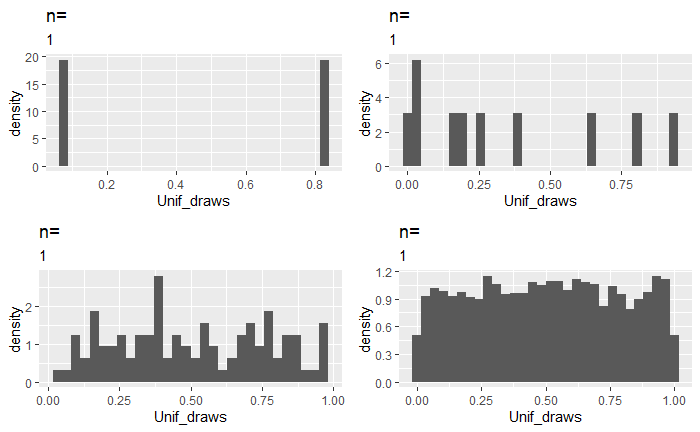
\includegraphics[width=0.7\textwidth]{0}
 \end{figure}  		   ~\\
 and indeed the larger the $S$ the closer the histogram to the PDF of Unif(0,1).\\~\\~\\

 \begin{minipage}{0.45\textwidth}
 	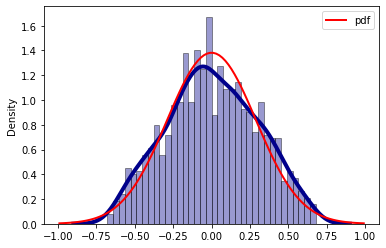
\includegraphics[width=0.9\textwidth]{1n2} \captionof{figure}{n=\textbf{2},S=1000}
 	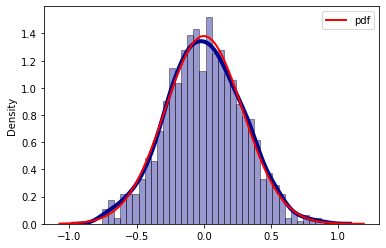
\includegraphics[width=0.9\textwidth]{1n20} \captionof{figure}{n=\textbf{20},S=1000}
 \end{minipage}
 \begin{minipage}[b]{0.45\textwidth}
 	From the comparison between the histograms of $X^*_n$ (blue) and normal density (red), we can see it indeed gets closer and closer as $n$ increases. \\~\\
 	Here we fix a large $S$ to make sure the histograms are good approximations for the density of $X_n^*$.
 \end{minipage}
\newline
Each line of code can be executed using $\text{ctrl}+\text{Enter}$ in Rstudio.
~\\~\\
This draws 4 values from Unif(0,1)
\begin{minted}[]{R}
runif(4, min = 0, max = 1)
\end{minted}
Here are the codes that you may find how many are the largest number
\begin{minted}[]{R}
rand.a=runif(4, min = 0, max = 1)
sum(rand.a==max(rand.a))
\end{minted}
We may repeat this game many many times and check how many more than 1 winner in S repeated games via the following codes:
\begin{minted}[]{R}
n=4;
S=100;
rand.Srepeats=matrix(runif(n*S, min = 0, max = 1),ncol=S)
colMax<- apply(rand.Srepeats, 2, max)
# this gives you the a True and false matrix, and only true if the max in that column
result=colMax==t(matrix(rep((colMax),n),nrow=S))
# how many more than 1 winner in S repeated games
sum(colSums(result)>1)
\end{minted}

Here we comparing the histogram of X*
(we generate S values drawn from the same distribution as the one of X* and then draw histogram)
with the density function of a normal distribution.
\begin{minted}[]{R}
set.seed(12)
require(ggplot2)
n=4
S=100
sigma2=1/12
# we generate S realised values of X* (simu_Sbar) by drawing from Unif distribution
simu_Sbar= colSums(matrix(runif(n*S, min = 0, max = 1)-1/2,ncol=S))/sqrt(n)

ggplot(data.frame(simu_Sbar), aes(simu_Sbar)) +
geom_histogram(aes(y=..density..)) +
stat_function(fun=function(x)1/sqrt(2*pi*sigma2)*exp(-(x)^2/sigma2/2),
color=rgb(0.6, 0.2, 0.2, 0.35), size=2)
\end{minted}

Here are also Python codes
\begin{minted}{python}
import numpy as np
np.random.seed(10)

# now again this draws 4 values from Unif(0,1)
np.random.uniform(0,1,4)

n=4;
S=100;
rand_Srepeats= np.random.uniform(0,1,n*S).reshape(-1,S)
# how many more than 1 winner in S repeated games
np.sum(np.sum(rand_Srepeats==rand_Srepeats.max(axis=0), axis=0)>1)


# X* distribution analysis
n=4
S=100
sigma2=1/12

rand_Srepeats= np.random.uniform(0,1,n*S).reshape(-1,S) -1/2
simu_Sbar= np.sum(rand_Srepeats.reshape(-1,S),axis=0)/np.sqrt(n)
#  Histogram
import seaborn as sns
sns.distplot(simu_Sbar, hist=True, kde=True,
bins=int(180/5), color = 'darkblue',
hist_kws={'edgecolor':'black'},
kde_kws={'linewidth': 4})

# we add some normal density
import math
ax=sns.distplot(simu_Sbar, hist=True, kde=True,
bins=int(180/5), color = 'darkblue',
hist_kws={'edgecolor':'black'},
kde_kws={'linewidth': 4})
# calculate the pdf
sigma2=1/12
x0, x1 = ax.get_xlim()  # extract the endpoints for the x-axis
x_pdf = np.linspace(x0, x1, 100)

y_pdf = 1/(np.sqrt(2*math.pi*sigma2))*np.exp(-np.power(x_pdf,2)/(2*sigma2))

ax.plot(x_pdf, y_pdf, 'r', lw=2, label='pdf')
ax.legend()
\end{minted}


\end{Solution}

% }

\end{document}
